\documentclass[mathserif]{beamer}

\usepackage{microtype}
\usepackage{xparse}
\usepackage{amsmath}
\usepackage{amssymb}
\usepackage{mathtools}
\usepackage{graphicx}

\frenchspacing

\logo{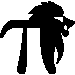
\includegraphics[width=0.07\textwidth]{../Logo}}

\usetheme{Rochester}
\usecolortheme{whale}

\setbeamertemplate{frametitle continuation}[from second][\hfill\insertcontinuationtext]

% Table of contents at start of each section
\AtBeginSection[] {%
	\begin{frame}
		\frametitle{Table of Contents}
		\tableofcontents[currentsection]
	\end{frame}
}

% Environments for math
\newenvironment{compactmath}[1][\normalsize]%
	{\begin{minipage}{\textwidth}\vspace{-0.5\baselineskip}#1\begin{equation*}}
	{\end{equation*}\end{minipage}}

\newenvironment{sizedmath}[1]%
	{\begingroup#1\begin{equation*}}
	{\end{equation*}\endgroup}

% Environments for consistent frame use
\newenvironment{namedframe}[1]%
	{\begin{frame}\frametitle{#1}\framesubtitle{\secname}}
	{\end{frame}}

\newenvironment{namedbreakframe}[1]%
	{\begin{frame}[allowframebreaks]\frametitle{#1}\framesubtitle{\secname}}
	{\end{frame}}

% Frames for emphasis
\newcommand{\sectionstart}[2]{\begin{frame}\frametitle{#1}\centering\Huge\secname\\\Large#2\end{frame}}
\newcommand{\bigframe}[1]{\begin{namedframe}{#1}\Huge\centering#1\end{namedframe}}

% Spacing commands
\newcommand{\sep}{\\\pause\vspace{1ex}}
\newcommand{\varsep}[1]{\\\pause\vspace{#1}}

\newcommand{\vertspace}{\\\vspace{1ex}}
\newcommand{\varvertspace}[1]{\\\vspace{#1}}

% Text formatting
\DeclareTextFontCommand{\emph}{\bfseries}

% Macros for math
\newcommand{\such}{\ |\ }
\DeclarePairedDelimiter{\ceil}{\lceil}{\rceil}
\DeclarePairedDelimiter{\floor}{\lfloor}{\rfloor}


\title{Introduction to the Fourier Transform}
\subtitle{Wave Voodoo}
\author{David Nash}
\institute{William Lyon Mackenzie C.I. Math Club}
\date{\copyright{} David Nash, 2018}

\begin{document}
	\frame{\titlepage}
	\section{Introduction}
	\begin{namedframe}{Background Knowledge}
		\begin{itemize}
			\item {Even/Odd Functions}
			\item {Periodic Functions}
			\item {Trigonometry}
			\item {Complex Numbers (and $e^{i\theta}$)}
			\item {Integration and IBP}
		\end{itemize}
	\end{namedframe}
	\begin{namedframe}{What is a Fourier Series?}
		\begin{itemize}
			\item {Decomposition of a periodic function into sines and cosines}
			\item {Expressed as $$\frac{a_0}{2}+\sum_{n=1}^{\infty}\left(a_n\cos\left(\frac{\pi nx}{L}\right) + b_n\sin\left(\frac{\pi nx}{L}\right)\right)$$}
			\item {or $$\frac{a_0}{2} + \sum_{n=1}^{\infty}a_n\sin\left(\frac{\pi nx}{L}+\phi_n\right)$$}
			\item {or $$\sum_{n=-\infty}^{\infty}c_ne^{i\frac{\pi nx}{L}}$$}
		\end{itemize}
	\end{namedframe}
	\begin{namedframe}{What is a Fourier Transform?}
		\begin{itemize}
			\item{Transformation of a function of time to a function of frequency}
			\item{Expressed as $$\hat{f}(\xi) = \int_{-\infty}^{\infty}f(x)e^{-i2\pi x\xi}\mathrm{d}x$$}
			\item{Exists both as \textit{continuous} and \textit{discrete} FT}
			\item{Today we will be looking at the former only}
		\end{itemize}
	\end{namedframe}
	\section{Fourier Series}
	\begin{namedframe}{Derivation of the Trigonometric Series}
		\begin{itemize}
			\item{For an even function:}
		\end{itemize}\pause
		\begin{align*}
			\action<+->{&f_e(x) = \sum_{n=0}^{\infty}a_n\cos\left(\frac{\pi nx}{L}\right)\\}
			\action<+->{&f_e(x)\cos\left(\frac{\pi mx}{L}\right) = \sum_{n=0}^{\infty}a_n\cos\left(\frac{\pi nx}{L}\right)\cos\left(\frac{\pi mx}{L}\right)\\}
			\action<+->{\int_{-L}^{L}&f_e(x)\cos\left(\frac{\pi mx}{L}\right)\mathrm{d}x = \int_{-L}^{L}\sum_{n=0}^{\infty}a_n\cos\left( \frac{\pi nx}{L} \right)\cos\left(\frac{\pi mx}{L} \right)\mathrm{d}x\\}
			\action<+->{&= \sum_{n=0}^{\infty}a_n\int_{-L}^{L}\cos\left( \frac{\pi nx}{L} \right)\cos\left(\frac{\pi mx}{L} \right)\mathrm{d}x\\}
			\action<+->{&= \sum_{n=0}^{\infty}a_n\int_{-L}^{L}\frac{1}{2}\left(\cos\left((m+n)\frac{\pi x}{L}\right) + \cos\left((m-n)\frac{\pi x}{L}\right)\right)\mathrm{d}x}
		\end{align*}
	\end{namedframe}
	\begin{namedframe}{An Aside}
		\begin{itemize}
			\item{Consider the integral $\int_{-L}^{L}\cos\left((m+n)\frac{\pi x}{L}\right)\mathrm{d}x$}
			\item{$$\frac{L}{m+n}\sin\left((m+n)\frac{\pi L}{L} \right) -\frac{L}{m+n}\sin\left((m+n)\frac{-\pi L}{L}\right) $$}
			\item{$$ = \frac{L}{m+n}\left( \sin((m+n)\pi) + \sin( (m+n)\pi)\right) = 0$$}
			\item{And so we have:$$\int_{-L}^{L}f_e(x)\cos\left( \frac{\pi mx}{L}\right)\mathrm{d}x = \frac{1}{2}\sum_{n=0}^{\infty}a_n\int_{-L}^{L}\cos\left((m-n)\frac{\pi x}{L}\right)\mathrm{d}x$$}
		\end{itemize}
	\end{namedframe}
	\begin{namedframe}{Another Aside}
		\begin{itemize}
			\item{For the reasons outlined last slide, $\int_{-L}^{L}\cos\left(\frac{(m-n)\pi x}{L}\right)\mathrm{d}x$ \textit{ usually} equals $0$}
			\item{However, if $m \equiv n$:}
			\item{$\int_{-L}^{L}\cos\left(\frac{(n-n)\pi x}{L}\right)\mathrm{d}x = \int_{-L}^{L}1\mathrm{d}x = 2L$}
			\item{EVERY other value of $m$ will yield a result of 0}
		\end{itemize}
	\end{namedframe}
	\begin{namedframe}{Conclusion}
		\begin{align*}
			\int_{-L}^{L}&f_e(x)\cos\left(\frac{\pi mx}{L}\right)\mathrm{d}x = \frac{1}{2}\sum_{n=0}^{\infty}\int_{-L}^{L}\cos\left(\frac{(m-n)\pi x}{L}\right)\mathrm{d}x\\
			&= \frac{1}{2}\left(0+0+\dots+0+0+2La_m+0+0\dots\right)\\
			&= La_m\\
			a_m &= \frac{1}{L}\int_{-L}^{L}f_e(x)\cos\left(\frac{\pi mx}{L}\right)\mathrm{d}x\\
			\therefore a_n &= \frac{1}{L}\int_{-L}^{L}f_e(x)\cos\left(\frac{\pi nx}{L}\right)
		\end{align*}
	\end{namedframe}
	\begin{namedframe}{Special Case: $n\equiv0$}
		\begin{align*}
			f_e(x) &= \sum_{n=0}^{\infty}a_n\cos\left(\frac{\pi nx}{L}\right)\\
			\int_{-L}^{L}f_e(x)\mathrm{d}x &= \sum_{n=0}^{\infty}a_n\int_{-L}^{L}\cos\left(\frac{\pi nx}{L}\right)\mathrm{d}x\\
			&= 2La_0 +0+0+0\dots\\
			\therefore a_0 &= \frac{1}{2L}\int_{-L}^{L}f_e(x)\mathrm{d}x\\
		\end{align*}
	\end{namedframe}
	\begin{namedframe}{Consolidation}
		\begin{itemize}
			\item{$b_n$ can be obtained just as easily, as: $$b_n = \frac{1}{L}\int_{-L}^{L}f_o(x)\sin\left(\frac{\pi nx}{L}\right)\mathrm{d}x\text{ }(b_0=0)$$}
			\item{A function neither even nor odd can be obtained via combination}
			\item{We can now express any periodic function as sines and cosines!\footnote{Restrictions may apply}}
			\item{$$f(x) = \frac{a_0}{2} + \sum_{n=1}^{\infty}\left(a_n\cos\left(\frac{\pi nx}{L}\right) + b_n\sin\left(\frac{\pi nx}{L}\right)\right) $$}
		\end{itemize}
	\end{namedframe}
	\begin{namedframe}{Exponential Form!}
		\begin{align*}
			\action<+->{f(x) &= \sum_{n=-\infty}^{\infty}c_ne^{i\frac{\pi nx}{L}}\\}
			\action<+->{f(x)e^{-i\frac{\pi mx}{L}} &= \sum_{n=-\infty}^{\infty}c_ne^{i\frac{\pi nx}{L}}\times e^{-i\frac{\pi mx}{L}}\\}
			\action<+->{\int_{-L}^{L}f(x)e^{-i\frac{\pi mx}{L}}\mathrm{d}x &= \sum_{n=-\infty}^{\infty} c_n\int_{L}^{L}e^{i(n-m)\frac{\pi x}{L}}\mathrm{d}x\\}
		\end{align*}
	\end{namedframe}
	\begin{namedframe}{An Aside (Look Familiar?)}
		\begin{align*}
			(n \not\equiv m)\text{ }\int_{-L}^{L}&e^{i(n-m)\frac{\pi x}{L}}\mathrm{d}x = \int_{-L}^{L}\cos\left( (n-m)\frac{\pi x}{L} \right)\mathrm{d}x \\&+ i\int_{-L}^{L}\sin\left( (n-m)\frac{\pi x}{L} \right)\mathrm{d}x\\
			= &\frac{L}{\pi(n-m)}\left(\sin( (n-m)\pi) - \sin(-(n-m)\pi)\right) \\&+ i\frac{L}{\pi(n-m)}\left( \cos( (n-m)\pi) - \cos(-(n-m)\pi)\right) = 0\\
			\text{OR ($n \equiv m$)}\\
			&= \int_{-L}^{L}\cos\left(0\right)\mathrm{d}x + i\int_{-L}^{L}\sin(0)\mathrm{d}x\\
			&= 2L\\
		\end{align*}
	\end{namedframe}
	\begin{namedframe}{Conclusion}
		\begin{align*}
			\int_{-L}^{L}f(x)e^{-i\frac{\pi mx}{L}}\mathrm{d}x &= 2Lc_m\\
			c_m &= \frac{1}{2L}\int_{-L}^{L}f(x)e^{-i\frac{\pi mx}{L}}\mathrm{d}x\\
			\therefore c_n &= \frac{1}{2L}\int_{-L}^{L}f(x)e^{-i\frac{\pi nx}{L}}\mathrm{d}x
		\end{align*}
	\end{namedframe}
	\begin{namedframe}{Recap}
		\begin{align*}
			f(x) &= \frac{1}{2L}\int_{-L}^{L}f(x)\mathrm{d}x + \sum_{n=1}^{\infty}\frac{1}{L}\int_{-L}^{L}\left(f(x)\cos\left(\frac{\pi nx}{L}\right)\mathrm{d}x\right)\cos\left(\frac{\pi nx}{L}\right)\\
			&\qquad+ \sum_{n=1}^{\infty}\frac{1}{L}\int_{-L}^{L}\left(f(x)\sin\left(\frac{\pi nx}{L}\right)\mathrm{d}x\right)\sin\left(\frac{\pi nx}{L}\right)
		\end{align*}
		\begin{align*}
			f(x) &= \sum_{n=-\infty}^{\infty}\frac{1}{2L}\int_{-L}^{L}\left(f(x)e^{-i\frac{\pi nx}{L}}\mathrm{d}x\right)e^{i\frac{\pi nx}{L}}
		\end{align*}
	\end{namedframe}
	
	\section{Fourier Transform}
	\begin{namedframe}{Setup}
		\begin{itemize}
			\item{Let $\xi = \frac{n}{2L}$ (The frequency of any term in the sequence), and extend $L$ to $\infty$.}
			\item{Now, \begin{equation*}c_n = \frac{1}{2L}\int_{-\infty}^{\infty}f(x)e^{-i2\pi x\xi}\mathrm{d}x\end{equation*}}
			\item{Just let $2Lc_n = \hat{f}(\xi)$, and that's our Fourier Transform!}
		\end{itemize}
		\begin{equation*}
			\hat{f}(\xi) = \int_{-\infty}^{\infty}f(x)e^{-i2\pi x\xi}\mathrm{d}x
		\end{equation*}
	\end{namedframe}
	\begin{namedframe}{Inverse Fourier Transform}
		\begin{itemize}
			\item{If $\xi = \frac{n}{2L}$, then let $\Delta\xi = \frac{1}{2L}$
		\begin{align*}
			\lim_{L->\infty}f(x) &= \lim_{L->\infty}\sum_{n=-\infty}^{\infty}\frac{1}{2L}\hat{f}(\xi)e^{i2\pi x\xi}\\
			&= \lim_{L->\infty}\sum_{n=-\infty}^{\infty}\Delta\xi\hat{f}(\xi)e^{i2\pi x\xi}\\
		\end{align*}
	}\item{But $\lim_{L->\infty} \frac{1}{2L} = 0$, and $\lim_{n->\pm\infty}\frac{n}{2L} = \pm\infty$}
		\end{itemize}
		\begin{align*}
			f(x) &= \lim_{\Delta\xi->0}\sum_{\xi=-\infty}^{\infty}\Delta\xi\hat{f}(\xi)e^{i2\pi x\xi}\\
			f(x) &= \int_{-\infty}^{\infty}\hat{f}(\xi)e^{i2\pi x\xi}\mathrm{d}\xi
		\end{align*}
	\end{namedframe}
	\begin{namedframe}{Disclaimer}
		\begin{itemize}
			\item{The Fourier Series only applies to \textit{piecewise continuous} functions}
			\item{The Fourier Transform is usually impossible to apply properly to functions over an infinite domain}
			\item{(Unless you're willing to teach yourself about the Dirac $\delta$ function)}
		\end{itemize}
	\end{namedframe}
\end{document}
